\documentclass{article}
\usepackage{fullpage}
\usepackage{amsmath,amssymb}
\usepackage{natbib}
\usepackage{marginnote}
\usepackage{graphicx}
\usepackage{hyperref}
\usepackage{latexml} % for \iflatexml

\newcommand{\var}{\mathop{\mbox{Var}}}
\renewcommand{\P}{\mathbb{P}}
\newcommand{\E}{\mathbb{E}}
\newcommand{\R}{\mathbb{R}}

\bibliographystyle{plain}

\begin{document}

\section{Introduction}

The covergent evolution of similar phenotypes in response to shared selection pressures is a testiment to the power of selection to repeatedly sculpt phenotypic variation. In some cases this convergence extends to the molecular level with dispate taxa converging to the same phenotype through parallel genetic changes in the same pathway, genes, or even by precisely the same genetic changes. 
Such precise convergence points to the conservation of function of the genes underlying adaptive traits, sometimes over deep time scales \citep{deephomologypapers}. Convergence on a molecular level also suggests that the path taken by adaptation can sometimes be relatively constained as few changes could have resulted in the adaptive phenotype, or that relatively few changes that can confer the advantagous phenotype of interest were sufficiently free of deleterious pleiotropic consequences to contribute to adaptation. 

%For highly polygenic traits 

Convergent adaptation can also occur within species, with individuals within a species 
adapted to the same environment in parallel through different large effect changes. 
There are a growing number of examples of this in a range of well studied organisms and phenotypes REFs.
All else being equal the evolution of convergent phenotypes within a species convergence is more likely with a higher mutational input, i.e. when the mutation target and population sizes are larger \citep{}. 
Convergence is also more likely when standing variation is present for the phenotype, 
as multiple pre-existing alleles can spread from low frequency, 
if our now adaptive alleles were previously not too deleterious \citep{Orr,Hermission}. 
When multiple rare changes sweep up from low frequency in parallel within a population this has been termed a soft sweep.\\

The geographic distribution of populations can also shape the probability of parallel mutation within a species.
A geographically wide spread species is more likely to adapt by multiple mutations im parallel if dispersal 
is geographically limited, as populations will adapt via new mutations rather than waiting for migration \citep{RalphCoop}. 
Convergence is also more likely if geographically separated populations adapting to similar environments 
via alleles which are maladapted in the environmentals separating them. 
Such adverse conditions can strongly spatially restrict the spread of locally adapted alleles \citep{lenormand} 
and so might encourage local adaptation by parallel mutation rather than migration.\\
 
For example a variety of plant species have repeatedly adapted to patchs of heavy metal soils
 (e.g. serpentine outcrops and mine tailings) within their ranges
and  alleles that adapt the plants to heavy metals may be disfavored off of these patches. 
Similarly across the American Southwest light colored rock pocket mice have adapted to outcrops of dark rock 
through the evolution of darker cryptic pigmentation. These dark outcrops are geographically
 separated by areas of light colored sand and rock, 
and strong selection appears to favour the matching of crypsis to substrate. 
Perhaps as a result of this strong selection against migrants, 
at least two distinct genetic changes are responsible from the dark pigmentation adaptation on different outcrops. 
This situation is repeated in XXXX where darker colored mice
 have repeated evolved lighter pigmentation to match lighter color sands on
 beaches via different genetic routes. 

%http://www.nature.com/hdy/journal/v94/n2/full/6800600a.html

In \citep{RalphCoop} we formulated a simple model of parallel adaptation in a geographic setting
where the selection pressure was constant across the entire environment, 
and that a single mutational change was sufficient to adapt populations to the novel environment. 
We assumed that there was no standing variation for the adaptive allele, such that parallel mutation must be due to multiple mutations after the environmental shift. In that setting we found that there was a characteristic geographic scale, over which we would expect multiple instances of our adaptive allele to have arisen in parallel. This characteristic length could be expressed in terms of a simple compound parameter determined by our parameters of interest.
Recall questions of origin of adaptations

References on parallel adapation, standing variation, etc.:
  coop,
  pennings and hermisson.
Note pennings and hermisson found standing deleterious variation was very important.  

recall peromyscus examples with patchy environments

Summarize previous paper

Question assumptions of no standing variation and homogenous selection

\section{Methods}
\subsection{Introduction to a patchily constructed model}
\label{ss:patchyspace}

Consider a population spread uniformly across a landscape. Within this environment there are patches of
habitat that individuals are initially poorly adapted to, surrounded by large areas that our population is well adapted to. 

It takes only a single mutational change to create an allele ($B$) that adapts an individual to the
poor habitat type. This mutational change occurs at a low rate of
$\mu$ per chromosome per generation. We assume that this initially rare new
allele has fitness $1+s_b$ relative to the unmutated type ($b$) in the ``poor'' habitat patches,
and assume that it has fitness $1+s_m$ when rare in the intervening areas, with
$s_m<0$. To simplify matters we assume that the disadvantage $s_m$ ensures that on the relevant timescale,
the allele is very unlikely to fix locally in the regions where it is at a disadvantage.

We are interested in the establishment of mutations in the ``poor'' patches by either
migration or mutation, and so we are only interested in whether the allele
can escape initial loss by drift when rare. Thus we do not have to
specify the the fitness of the homozygote, only that its
fitness is such the dynamics of the  allele when it is rare are
determined by the fitness of the heterozygote. This allows us to treat
a diploid model as being essentially haploid for our purposes. \gc{TRUE?}

For the sake of simplicity we will assume a constant haploid population density $\rho$, 
across both types of habitat (we will return to discuss this equal
density point later). We further assume that the
variance in offspring number is $1$, and that the mean squared distance between parent and child is $\sigma^2$ (the dispersal variance).

As only a single mutation is required to adapt individuals to the
poor habitat patch, subsequent mutations that arise after an allele
becomes established at its equilibrium frequency on the patch gain no selective
benefit. Similarly an allele introduced into a patch by migration will
not be favored by selection to spread, if the patch has already been
colonized. Thus mutations selective exclude each other from
patches, over short-time scales, and they will only slowly filter
together over longer time scales by drift. 

\paragraph{Previous work} We will make use of a number previous
results from the literature. \citet{slatkin1973geneflow}, working in
one dimensional deterministic framework, showed that if the
physical width of the patch is less than $2 \tan^{-1}
(\sqrt{|s_m/s_b|})$, then $B$ can not 
become stably established within the patch, as the local adaptation prevented by
migrational swamping \citep[see also][ for a review]{Lenormand}.
 \citet{barton1987establishment}, again working in one dimension,
 showed that this critical patch size also held in a stochastic
 framework \citep[see also the work of][]{Polk}. 
For patches above this size, \citet{barton1987establishment}
 founds that mutations appearing further than a few multiples of
 $\sigma/\sqrt{2|s_m|}$ away from such a patch have vanishingly small
 probability of becoming established within the patch. 
Barton also showed that mutations appearing within the patch have probability 
strictly less but approaching that $2s_b$ of establishment as the size
of the patch increased. Thus for large enough patches the probability
of establishment of a locally favorable allele approaches the standard
establishment probability ($2s_b$) for a panamitic population
\citep[][]{haldane, fisher}, a result that also (generally) holds for
a geographically spread population experiencing a uniform selection
pressure \citep{Maruyama, cherry}. 

%Maruyama: On the fixation probability of mutant genes in a subdivided population*

%To make things tractable, we assume that the distances between the patches are large relative to migration distance $\sigma$,
%and that the disadvantage $s_m$ ensures that on the relevant timescale,
%the allele is very unlikely to fix locally in the regions where it is at a disadvantage.


%A similar situation of interest is the case when the species occupies a continuous range, but the selective pressure itself is patchy.
I%f the areas where the new allele is advantageous are relatively isolated,
%we might hope to apply the results above to such a situation.
%For this purpose, suppose that instead of a uniform habitat,
%the selective pressure is such that the new alleles are only advantageous in isolated locations, 
%and are disadvantageous in the intervening region.
%As before, we assume that the new allele has fitness $1+s_b$ relative to the unmutated type in the ``good'' patches,
%and assume that it has fitness $1+s_m$ in the intervening areas, with $s_m<0$.
%To make things tractable, we assume that the distances between the patches are large relative to migration distance $\sigma$,
%and that the disadvantage $s_m$ ensures that on the relevant timescale,
%the allele is very unlikely to fix locally in the regions where it is at a disadvantage.
%With these assumptions as justification, we will move to a model of discrete demes exchanging migrants,
%where ``migration'' occurs through the rare, transient passage of the new allele through regions where it is disadvantageous.

%equal deme sizes?  general migration rates?

\subsubsection{Mutational influx}
\label{ss:patchymutation}
Consider first a single, isolated poor habitat patch of area $A$ in
which no $B$ allele has yet become established. As
we are interested in local adaptation that can occur we will assume
that our patch is considerably larger than the cutoff for local
establishment, i.e. $\sqrt{A} \gg 2 \tan^{-1} (\sqrt{|s_m/s_b|})$.

Let $p(x)$ be the probability that a new allele arising at location
$x$ away from the patch fixes within the poor habitat patch.
The function $p(x)$ can be found in terms of Jacobi elliptic functions,
XXX as shown in the Appendix, but the expressions are particularly unhelpful.
The total successful mutational influx per generation is then given by $\int \rho \mu p(x) dx$,
and depends in a complicated way on the relationship of patch width and selection coefficients,
but still scales linearly with the population mutational influx $\rho \mu$.
Therefore, we define $p_f = \int p(x) dx$.  If the width of the patch, $\sqrt{A}$, is large
relative to $\sigma/\sqrt{2s_m}$ then a reasonable approximation is to
set $p_f \approx 2 s_b A$. This follows from the fact that if the
patch is large than the majority of the mutations that could become
established within the patch, arose within the patch.  


The rate at which mutations arise and colonize the patch is on the order of $\rho \mu
p_f$ generations, which will approximately be $2 s_b \rho \mu$. If
this rate is low,  then the waiting time till a mutation arises that
will become locally established within the patch is exponentially
distributed with mean $2 s_b \rho \mu$.  Assuming that once a mutation
becomes established
 it quickly reaches its equilibrium frequency across the patch, the
 expected time it takes for our patch to become colonized by the $B$
 allele is $1/(2 s_b \rho \mu)$.


\subsubsection{Migration rates}
\label{ss:patchymigration}

Now suppose that there are two patches, each of area $A$, of the poor
habitat type separated by distance $R$. Consider the case where the
allele has arisen and become established in the first patch, but has not yet appeared in the second.
As above, any copy of the new allele that appears at location $x$ relative to the second, unadapted patch 
has probability approximately $p(x)$ of fixing locally in this patch,
whether the allele is a new mutation or is descended from the occupants of the first patch.
Due to mutation--selection balance there will be a small number of alleles descended from those of the first patch (``migrants'') 
present in the regions where they are disadvantageous;
the equilibrium frequency may again be expressed in terms of Jacobi elliptic functions (Appendix XXX, citeXXX),
although the equations are again not particularly helpful.
However, we do know that if $q(r)$ is the expected proportion present at mutation--selection balance at distance $r$ from the first patch
in the absence of the second patch, that for large $r$ the proportion decays exponentially, $q(r) \approx C \exp( -|\sqrt{s_m} r / \sigma|)$,
where $C$ is a constant depending on the structure of the populations and the selection coefficients.

Combining this with the calculations above allows us to get a rough sense of the scale of migration between separated patches,
supposing that patches are large enough for local fixation to be
stable. If the alleles were not advantageous in the second patch,
the average numbers of mutant alleles present near the second patch would be around $\rho A \exp( - |\sqrt{s_m} R/\sigma| )$;
so the waiting time until some migrant allele fixes in the second patch would be something like $T_m = ( 2 s_b \rho A \exp( - |\sqrt{s_m} R/\sigma|)^{-1}$.
If $T_m$ is large, then we would expect successful migrants to be rare,
so that if the second patch adapts through migration, it is likely to come from only a single migrant.
We leave aside the converse situation, for which there is likely to be more than one migrant
that founds the population mutant individuals in the new patch.


\subsection{Patchy Selection -- Results} 
\label{ss:discreteresults}

We will assume that once a mutation escapes loss and becomes
established in the poor habitat patch it reaches its equilbrium frequency very rapidly. 


If environment is continuous, with separated patches where the new allele is advantageous,
we can only get a rough sense of whether the new adaptation is likely to spread through mutation (i.e.\ in parallel)
or through migration.
Taking the expressions from sections \ref{ss:patchymutation} and \ref{ss:patchymigration} above,
we see that if patches each have sufficiently large area $A$,
then the mutational input in each is on the order of $2 \rho \mu A$,
while the influx due to migration between patches separated by distance $R$ is on the order $2 \rho A \exp(- |\sqrt{s_m} R/\sigma|)$. 
If the input from mutation and migration are comparable, i.e.\ if $\mu \approx \exp( -|\sqrt{s_m} R/\sigma| )$,
then adaptation is expected to take place both by migration and mutation.
If we take $\mu = 10^{-8}$, then this is satisfied if $R/\sigma \approx 18/\sqrt{s_m}$.
so if the disadvantage to the new mutation between patches is fairly strong (say, $s_m=.05$),
then the distance between patches must be about a hundred times the dispersal distance (i.e.\ $R/\sigma \approx 100$);
while if $s_m$ is much smaller, say $s_m = .001$, 
then the patches must be separated by many hundreds of times the dispersal distance (i.e.\ $R/\sigma \approx 500$).
The situation does not change much if $\mu$ is larger -- even if $\mu = 10^{-6}$, 
the required separation between patches is only reduced by 60\%.
If the separation between patches is much larger -- say, by a factor of ten -- 
then patches are effectively isolated -- most adaptation will be independent between patches.
On the other hand, if the separation is much smaller, then a single mutation is likely to fix everywhere.

Furthermore, in the model of discrete demes connected by symmetric weak migration, 
the final distribution of types depends only on the ratio of mutation to migration rates,
and that the number of independently arisen types follows the Ewens distribution, with parameter $\mu/m$.
In Figure \ref{fig:discbyratio} we plot mean number of types and size (number of demes occupied) of a sampled type,
for a model with 20 interconnected demes, across different parameter values.  
This indicates that we need the population-scaled mutation and migration rates 
to be within a factor of about 100 of each other for parallel adaptation to leave an interesting pattern.  
If migration is faster, then a single type is likely to take over, while if migration is weaker, each deme is likely to come up with its own type.

\begin{figure}[ht]
 \begin{center}
   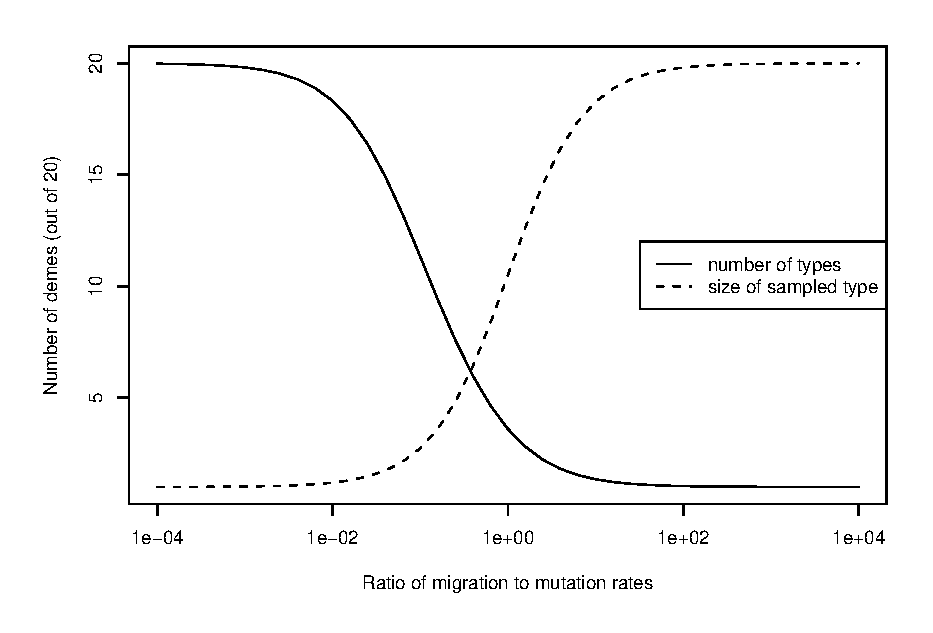
\includegraphics{discrete-by-ratio}
 \caption{ %
 The mean number of types and the mean number of demes occupied by a sampled type, in a discrete model with 20 demes,
 plotted as a function of the ratio of migration to mutation probabilities.
 Note the log scale on the horizontal axis.
 \label{fig:discbyratio}
 }
 \end{center}
\end{figure}

Also note that the properties of the discrete model are independent of the {\em sizes} of the demes themselves--- we have assumed away all such dependence.
This is complementary to the results of \cite{softsweepsII}, who showed that multiple mutations are likely to arise {\em within} a panmictic deme
if the population-scaled mutation rate $2 N \mu$ is greater than $1$.

\section{Applications} 

HbS

lava bed peromyscus

G6PD

\section{Discussion} 

if populations and mutation rates are large enough, parallel adaptation is likely, aided by geography. 
recall others' work. 

patchy selection helps this happen; 
effective migration rate looks like what; 
strength of (positive?) selection suprisingly does not affect results (?) 

standing variation will be important under these circumstances; 
migration rate (and so geographic structure) will not affect numbers of types if this is true; 
however migration always affcts spatial patterns. 

discussion of applications. 

discuss mixing of types; 
Graph: from simulation showing local proportions in a single patch showing initial fixation of a single type and later mixing converging toward more than one type.  (and eventual loss of one?)

\bibliography{standing_patches_refs}

\appendix

\section{Integrals appearing in the text}
    \label{apx:integrals}

In the text at several points appear integrals of the form
\begin{align}
  \int_0^\infty t^c \exp \left( - \alpha t^d - \beta t^{d+1} \right) dt 
\end{align}
where $c$ is a positive integer, $d$ is the dimension, and $\alpha$ and $\beta$ are positive real numbers.
This could be evaluated through standard numerical methods; below we describe a power series expansion.
Changing variables to $u = \beta t^{d+1}$, this becomes
\begin{align}
    \left( (d+1)^{-1} \beta^{ (1-c)/(d+1) } \right) \int_0^\infty u^{(c+1-d)/(d+1)} \exp\left( - \alpha \beta^{-d/(d+1)} u^{d/(d+1)} - u \right) du ,
\end{align}
so it suffices to evaluate the function
\begin{equation}
    G(a,b,x) := \int_0^\infty  t^a \exp\left( -x t^b - t \right) dt ,
\end{equation}
in the case that $a=(c-d+1)/(d+1)$, $b=d/(d+1)$, and $x$ is a function of the demographic paramters.
Since $a$ and $b$ only depend on the dimension and the quantity being computed,
we are interested in $G$ as a function of $x$.
At least in the case $b=d/(d+1)$ it is possible to express $G$ as a finite sum of gamma functions,
but we proceed with a simpler method.
Note that $\partial_x G(a,b,x) = -G(a+b,b,x)$,
and that at $x=0$, the function $G$ is the gamma function $G(a,b,0) = \Gamma(a+1)$.
Therefore, a Taylor series for $G$ would be
\[
    G(a,b,x) = \sum_{n \ge 0} = \sum_{n \ge 0} \frac{(-x)^n}{n!} \Gamma(a+nb+1) .
\]
It is easy to check using Stirling's formula that $\limsup_{n \to \infty} ( x^n \Gamma(a+nb+1)/n! )^{1/n} = 0$
if $b<1$, so the sum converges.


\section{Patchy selection} 
\label{ss:discretedemes}

We have been working in a continuous model of geographic space; 
in this section we move to a discrete model of isolated populations exchanging rare migrants,
but in section \ref{ss:patchyspace} discuss how a model with {\em patchy} selection can be approximated by such a discrete model.

Suppose now that we have a set of $L$ discrete populations of individuals that may reproduce or migrate,
and that migration and mutation are rare, so that the waiting times until either event is approximately exponential.
Suppose that for each pair of populations, labeled $i$ and $j$, the mean number of migrants that travel from $i$ to $j$ per generation
is $M_{ij}$ and that the mean number of new mutations appearing in population $i$ per generation is $\mu_i$.

{\tt Include cartoon here.}

If we suppose that fixation occurs on a faster time scale than mutation or migration,
so that it is very unlikely that two different migrants or mutants begin to fix locally in the same population,
then we can treat the process of extinction or local fixation as instantaneous 
(a limit previous studied by \cite{Slatkin:81}).
In this limit we may also ignore swamping effects of inmigration of nonmutant alleles.

In this case, we have the following picture.
The population at first starts out with no selected alleles. 
At some later time point suppose that there are $T$ different alleles present in the population, 
that the $k^\mathrm{th}$ allele is occupying demes $\{i^k_1, \ldots, i^k_{n_k}\}$, for $1\le k \le T$.
Let $I$ denote the set of all adapted demes, 
and let $J = \{j_1, \ldots, j_\ell\}$ denote the demes that have not yet adapted, with $\ell = L - \sum_k n_k$.
Then we are assuming that two types of event can happen which could change the state:
either at rate $\mu_j p_f$, an unadapted deme $j$ produces a new mutant, which fixes in this deme;
or at rate $M_{ij} p_f$, an adapted deme $i$ sends a migrant to unadapted deme $j$, which fixes in that deme.
Therefore, under these assumptions, the probability of fixation $p_f$ (and hence the selection coefficient)
only enter as a time scaling: for instance,
if we define $R = \sum_{j \in J} \left( \mu_j + \sum_{i \in I} M_{ij} \right)$,
then the total rate of such events is $p_f R$.
The probability that the next event results in, say, adaptation of deme $j$
is 
\[
 \left( \mu_j + \sum_{i \in I} M_{ij} \right) / R,
\]
and the probability that deme $j$ adapts through migration from deme $i$, given that deme $j$ is the next to adapt, is
$M_ij / R$,
while the probability that it adapts through a new mutation is $\mu_j / R$.

The main point here is that the final pattern,
and hence the likely extent of parallel adaptation,
is independent of the strength of selection.
This is in contrast to the continuous case, however, this observation is dependent on the assumption of weak migration
and fails to hold if different migrant lineages interact.
This can be viewed as a continuous-time Markov process XXX.
Explicit solutions are not available in the general case,
but if we specialize to a completely symmetric model (i.e.\ the ``island'' model),
then the mathematical picture is a pretty one.

\subsection{Symmetric patches}

Indeed, suppose that migration and mutation are symmetric: $M_{ij}=m$ and $\mu_j = \mu$ for all $j$ and $i\neq j$.
Suppose at some time the $k^\mathrm{th}$ allele is occupying $n_k$ demes, 
with $n = \sum_k n_k < L$.
Then at rate $(L-n) N \mu p_f + n (L-n) N m p_f$,
either a migration or mutation event happens.
With probability $\mu/(\mu + n m)$, it is a mutation,
and a new deme is randomly chosen and assigned a new allele.
With probability $n_k m / (\mu + n m)$,
the $k^\mathrm{th}$ type sends a successful migrant to a randomly chosen new island,
which is assigned the $k^\mathrm{th}$ allele.

This process is a continuous-time version of the ``Chinese restaurant process''
described in \citet{aldous1985exchangeability} and \citet{pitman1995partitions},
and so the final partition of types across demes has the Ewens sampling distribution with parameter $\mu/m$.
Again note that the selection coefficient, which is implicit in the probability $p_f$,
does not enter into the final distribution.

Now we can compute most properties we might want about the process.
For instance, the expected number of distinct mutational origins is
\begin{equation}
    \E\left[ \mbox{ \# of independent mutations } \right] = 
            1 + \frac{\mu}{m} \sum_{k=2}^L \frac{1}{k+(\mu/m)}. \label{discrete_expected}
\end{equation}
The probability that there is only a single successful mutation is
\begin{equation}
\P \left\{ \mbox{only one mutational origin} \right\} = 
            \prod_{k=1}^{L-1} \frac{ k }{ k+(\mu/m)} .
\end{equation}
More generally, suppose we sample a single deme, and are interested in the total number of demes $S$
(including the sampled one) that share the same fixed mutation as our sampled deme.
Then $S$ has distribution
\begin{equation} \label{eqn:Sdistrn}
\P\{ S=s \} = \frac{ (s-1)! (\mu/m)^{L-s} }{ \prod_{k=1}^{L-1} (k+(\mu/m)) } .
\end{equation}
Furthermore, if $L$ is large, then $S/L$ has probability density approximately
\begin{equation} \label{eqn:betadistrn}
   (\mu/m) (1-x)^{(\mu/m)-1}
\end{equation}
namely, is a $\mathrm{Beta}((\mu/m), 1)$ distribution--- see \cite{donnelly-joyce} and \cite{permanPitmanYor92}.

% In Figure \ref{fig:discbyratio} we plot mean number of types and size (number of demes occupied) of a sampled type,
% for a model with 20 interconnected demes, across different parameter values.  
% This indicates that we need the population-scaled mutation and migration rates to be within a factor of about 100 of each other for parallel adaptation to leave an interesting pattern. If migration is faster, then a single type is likely to take over, while if migration is weaker, each deme is likely to come up with its own type.

The high connectedness of the discrete deme island model means that the expected number of distinct alleles, (Equation \eqref{discrete_expected}), 
grows with the $\log$ of the number of demes. This strongly contrasts with the continuous spatial model where the local nature of dispersal means that doubling the species range will double the number of mutations expected. 
Furthermore, while in the continuous model the areas occupied by distinct mutations are similar in area, in this strong-selection discrete island model, 
only a few types tend to dominate even as the number of demes (and thus, distinct types) grows large (see Equations \eqref{eqn:Sdistrn} and \eqref{eqn:betadistrn}).

A more general model would allow migration only along edges of some graph connecting the demes.
In the low migration limit such a model still produces a partition distribution independent of the selection coefficient,
but it does not in general have the Ewens distribution.
Another extension would be to include the time alleles need to achieve an intermediate frequency,
along the lines of \citet{Navarro:03}, which would reintroduce dependence on the selection coefficient.

\texttt{XXX omit this? XXX}
We have treated the time during which the selected allele is at intermediate frequency in a deme (about $\log(\sigma^2 \rho)/s_b$ generations) as negligible, 
which ignores migration events that occur while the mutation is spreading through the population. 
we now sketch of a more realistic approximation.
For each occupied--unoccupied pair of demes, if the number of mutant alleles in the occupied deme is $n(t)>0$,
then at time $t$, migrants from the occupied deme pass the selected allele to the unoccupied deme at rate $2 n(t) m p_f(s_b)$,
while newly arisen mutants arise and fix in the unoccupied deme at constant rate $2 N \mu p_f(s_b)$.
The selected type should grow approximately as $n(t)=\exp(s(t-t_0))$.
Of course, to follow this model through, we will have to account for multiple types within a single deme and other complications,
but we can at least make a few observations.
One is that the final distribution of types is no longer independent of $s_b$, which enters through the dynamics $n(t)$.
However, it is clear that increasing the selection coefficient $s$ will decrease the number of types (independent mutational origins),
while on the other hand, increasing the deme size $N$ will increase the number of types,
and that the case presented above is at the extreme (see also \cite{Navarro:03} for deterministic approximations). 


\end{document} 
